%!TEX TS-options = -shell-escape
\documentclass[oribibl]{llncs}
\usepackage{makeidx}  % allows for indexgeneration

\usepackage[utf8]{inputenc}
\usepackage{pdfpages}

% \usepackage[nottoc,numbib]{tocbibind}
% \usepackage[center]{caption}

\usepackage{enumitem}
%\usepackage[margin=1.5in]{geometry}
\usepackage{url}
\usepackage[multiple]{footmisc} % DOUBLE FOOTNOTES ACROSS THE SKY
\renewcommand{\footnotemargin}{3.99pt}

% %% to make urls look better in bibliography
% \makeatletter
% \def\url@leostyle{%
%   \@ifundefined{selectfont}{\def\UrlFont{\sf}}{\def\UrlFont{\small\ttfamily}}}
% \makeatother
% %% Now actually use the newly defined style.
% \urlstyle{leo}

\bibliographystyle{plain}



\begin{document}

% insert the table of contents if want, it is not required
% llncs says: "If you are the author of a single contribution you
% normally have no running heads and no table of contents."
% \tableofcontents

\mainmatter              % start of the contributionsmainmatter
\title{Point Location in Voronoi Diagrams}

\author{Anders Høst Kjærgaard \and Hildur Uffe Flemberg\\
\email{\{ahkj, hufl\}@itu.dk}}

% Do we want to show our emails?
\institute{IT University of Copenhagen, Rued Langgaards Vej 7, 2300 Copenhagen S, Denmark}


\maketitle              % typeset the title of the contribution

\begin{abstract}
Voronoi diagrams are used in a variety of contexts in mathematics, biology and computing. We are interested in analysing the composition of the voronoi diagram to say something  about the underlying data that the diagram represents. In this paper we descibe a solution that generates a voronoi diagram from an arbitrary set of data points and returns a data structure for performing point location i O(log n) time in the generated diagram. The solution makes use of an existing open-source implementation of Fortunes algorithm for generating voronoi diagrams, which is merged with our own implementation of a trapezoidal map for performing point location. Querying the trapezoidal map data-structure will return the site of the voronoi cell in which the query point lies.  Secondly, we use the point location as basis for an analysis of the expected number of query points that will end in the biggest voronoi cell when distributed randomly across the diagram. We discuss why performing point location on Voronoi diagrams could of interest in various domains.

\begin{figure}[t]
    \centering
      
\includegraphics[height=80mm]{images/voronoi_diagram.pdf}
    \caption{A Voronoi Diagram with 15 sites}
    \label{fig:Pipes2IFCWorkflow}
\end{figure}


\keywords{algorithms, computational geometry, point location, software development}
\end{abstract}

% Number the first pages with Roman numbers
\pagenumbering{roman}

 %!TEX root = ./report.tex


% Slides:
% - General statement introducing the area; You can most likely start with the first paragraph from your project description and evolve it.
% - Explanation of the specific problem and why do we care about the problem.
% - Explanation of your solution, and how it improves on the work by others. Relation to related work can be very brief, given that you have a separate extensive section devoted to this.
%  -A hint on how the solution was evaluated and what was the outcome of this evaluation.
%  -A summary (a “map”) of how the paper is organized.

\pagenumbering{arabic}
\setcounter{page}{1}
\section{Introduction}
\label{introduction}
This report is written at the IT University of Copenhagen in the fall term of 2012 in connection with the Algorithm Design 2 project supervised by Rasmus Pagh. In the following pages we define an algorithmic problem, give examples of domains where this problem could be found and provide a solution to it. The solution is based on the concept of Voronoi diagrams and the problem of finding an area in a planar subdivision that contains a specific point.
The reader of the report is not assumed to have any prior knowledge of Voronoi diagrams or point location. However, we recommend to study the literature from the references as the project is based on these and we will only present the main concepts.

A planar subdivision is a division of a two-dimensional surface into non-overlapping cells. An example of this, maps can be divided into regions of longitude and latitude intervals. Given a geographic position (a query point), a point location query in a map would return the cell that contains the query point. Such queries could be useful for retrieving information abaout a given ares, say currents in the water, location specific weather forecasts or simply which country you are in. 

A Voronoi diagram is a special case of a planar subdivision created from a set of points of interest – normally referred to as $sites$. Every cell in a Voronoi diagram contains exactly one site. Furthermore, every point inside the cell of a site $S$, share the property that they are closer to $S$ than to any other site in the diagram. By extension every point that lies on the boundary of two or more Voronoi cells are equidistant from the sites of the neighbouring cells. Due to these rather generic properties, Voronoi diagrams have found applications within a big number of domains including biology, mathematics, geography and route planning to name a few.\cite{voronoi_applications} \paragraph{}
In this report we focus on the domain of fast food restaurants, i.e. we seek to answer queries that might be relevant to a chain of restaurants like McDonalds or to a customer. Examples of such queries could be “What would be a good location for us to place a new restaurant?” or from the view of a customer “What is the nearest fast food restaurant?”. When answering these queries, we will make enough assumptions about the domain to be sure that a deterministic answer exists.
%!TEX root = ./report.tex
\section{Background}
\label{background}

In this section, we provide some background information on Fortune's algorithm for generating Voronoi diagrams, and the trapezoidal map algorithm for point location, which we will later merge into one.

\subsection{Fortunes Algorithm}
Fortune’s algorithm is a sweep line algorithm that generates a Voronoi diagram from a set of sites given as input. By sweeping a horizontal line from top to bottom of all the sites the algorithm is capable of determining the position of all vertices and edges in the diagram. The output is a doubly connected edge list (DCEL) corresponding to the edges of a Voronoi diagram.

\paragraph{}
In general, the edges of a Voronoi diagram can be full lines, meaning that they have one or zero endpoints, or they can be true line segments. To be able to store the edges of the result in a DCEL, the algorithm outputs all edges as segments. This is achieved by assuming that all sites are contained in a bounding rectangle that cuts off the lines that would otherwise be unbounded.

To compute the diagram, the algorithm sweeps from the top of the rectangle and terminates when it reaches the bottom. During the sweep, two kinds of events can happen. 

\subsubsection{Site events}
occur when the sweep line reaches a new site. After a site event it is possible to define a parabola with its narrow end pointing downwards, and the site that caused the event as its focal point. When this happens, all the points that lie inside the parabola will be closer to the newly discovered site than to any other site lying below the sweep line. As soon as the sweep line reaches the next site, a new parabola will be created and so on. A snap shot of the algorithm in progress can be seen in Figure~\ref{fig:fortunes}.

\begin{figure}[]
    \centering
      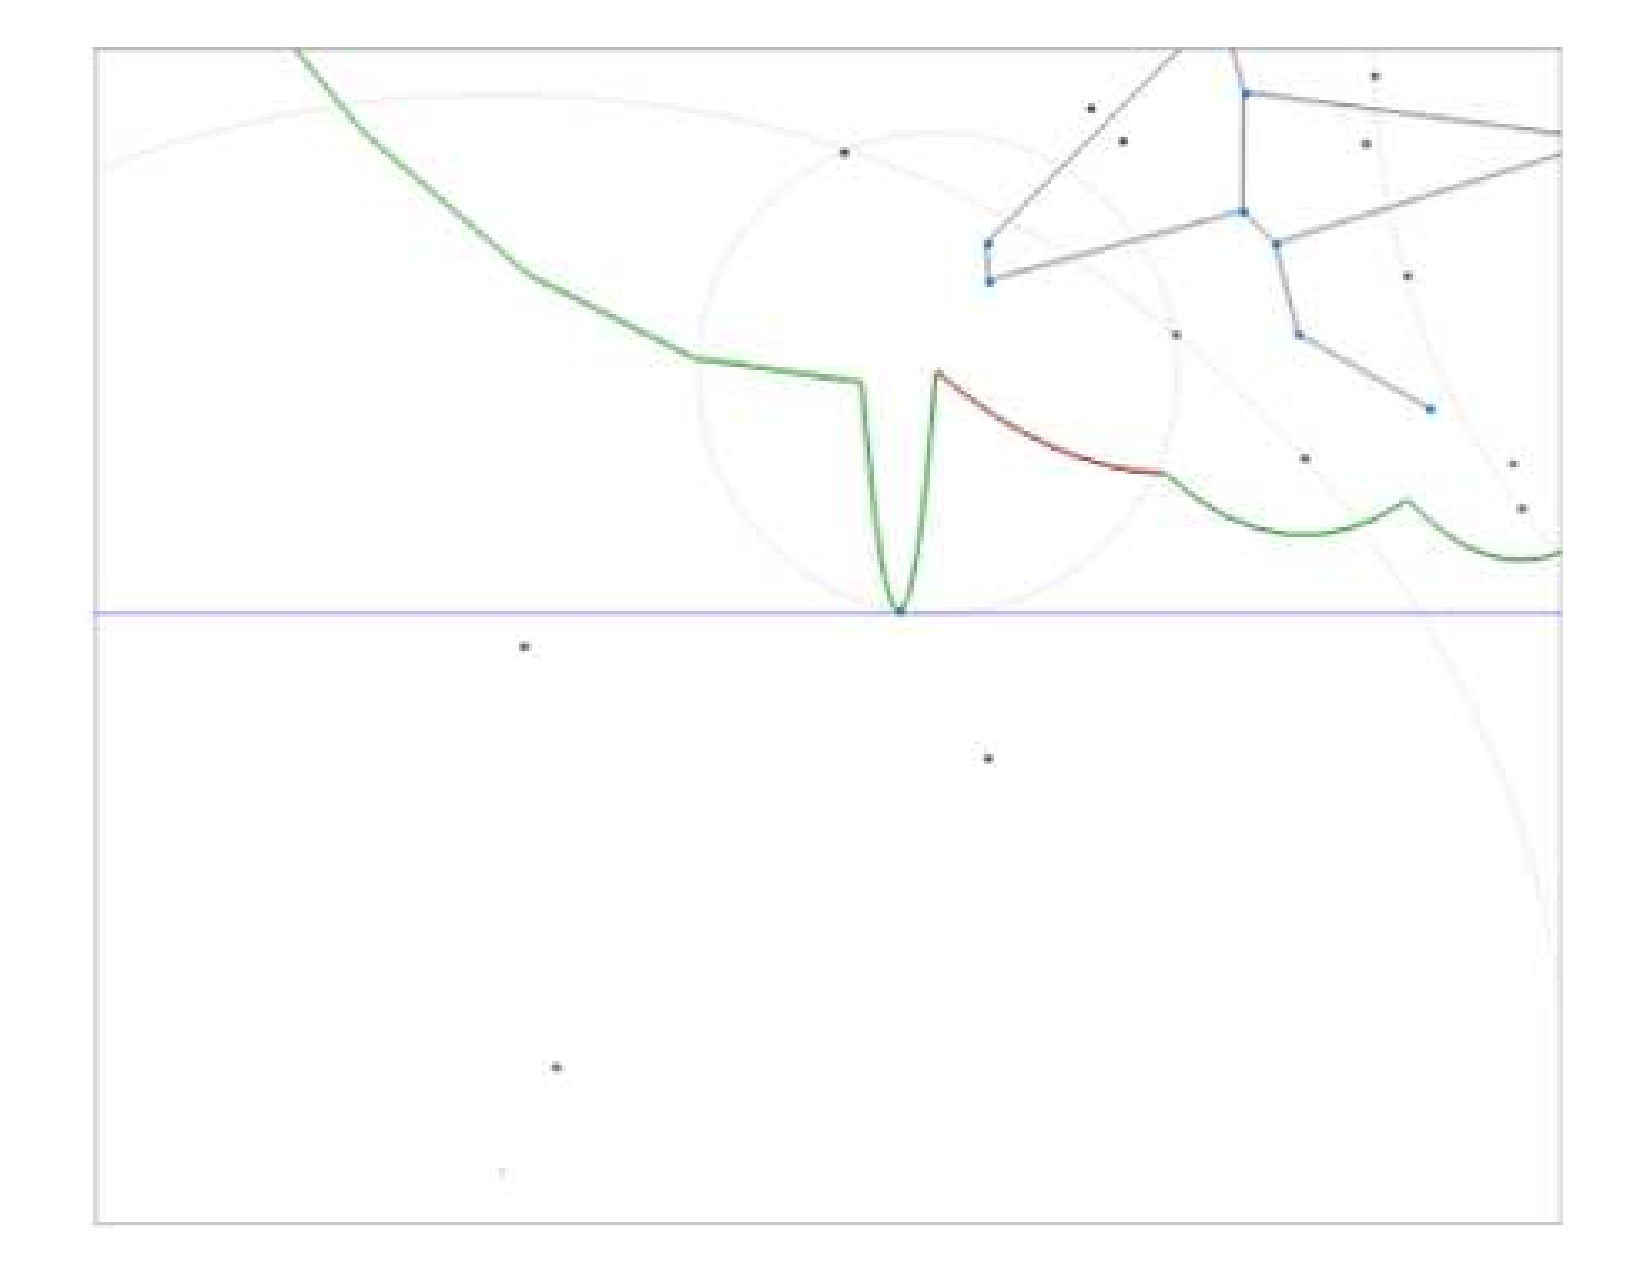
\includegraphics[width=80mm]{images/fortunes.pdf}
    \caption{Snapshot of Fortune's algorithm. A site event has just occured on the sweep line, and a few line segments and vertices have been discovered in the upper right corner. Below the sweep line we see 3 future site events.}
    \label{fig:fortunes}
\end{figure}

\paragraph{}
Since the points that form the intersections between two parabolas are equidistant to the sites represented by their respective parabolas, these intersections must be part of the final Voronoi diagram, by definition. Since the size of the parabolas depend on the location of the sweep line, they will widen as the sweep line advances its position. The intersections will move as well and trace out the line segments of the Voronoi diagram. Initially, when the sweep line is in the horizontal position of the new site, the parabola is just a vertical line crossing the site.

\subsubsection{Circle events}
occur when the sweep line reaches a position where it acts as a horizontal tangent to a circle that also intersects three sites above the sweep line. At that moment, a situation has occurred where three points with known positions are equidistant to the centre of the circle. Since the centre of the circle is equidistant from more than two points, it becomes a vertex in the Voronoi diagram. The situation is shown in Figure~\ref{fig:circle_event}.

\begin{figure}[]
    \centering
      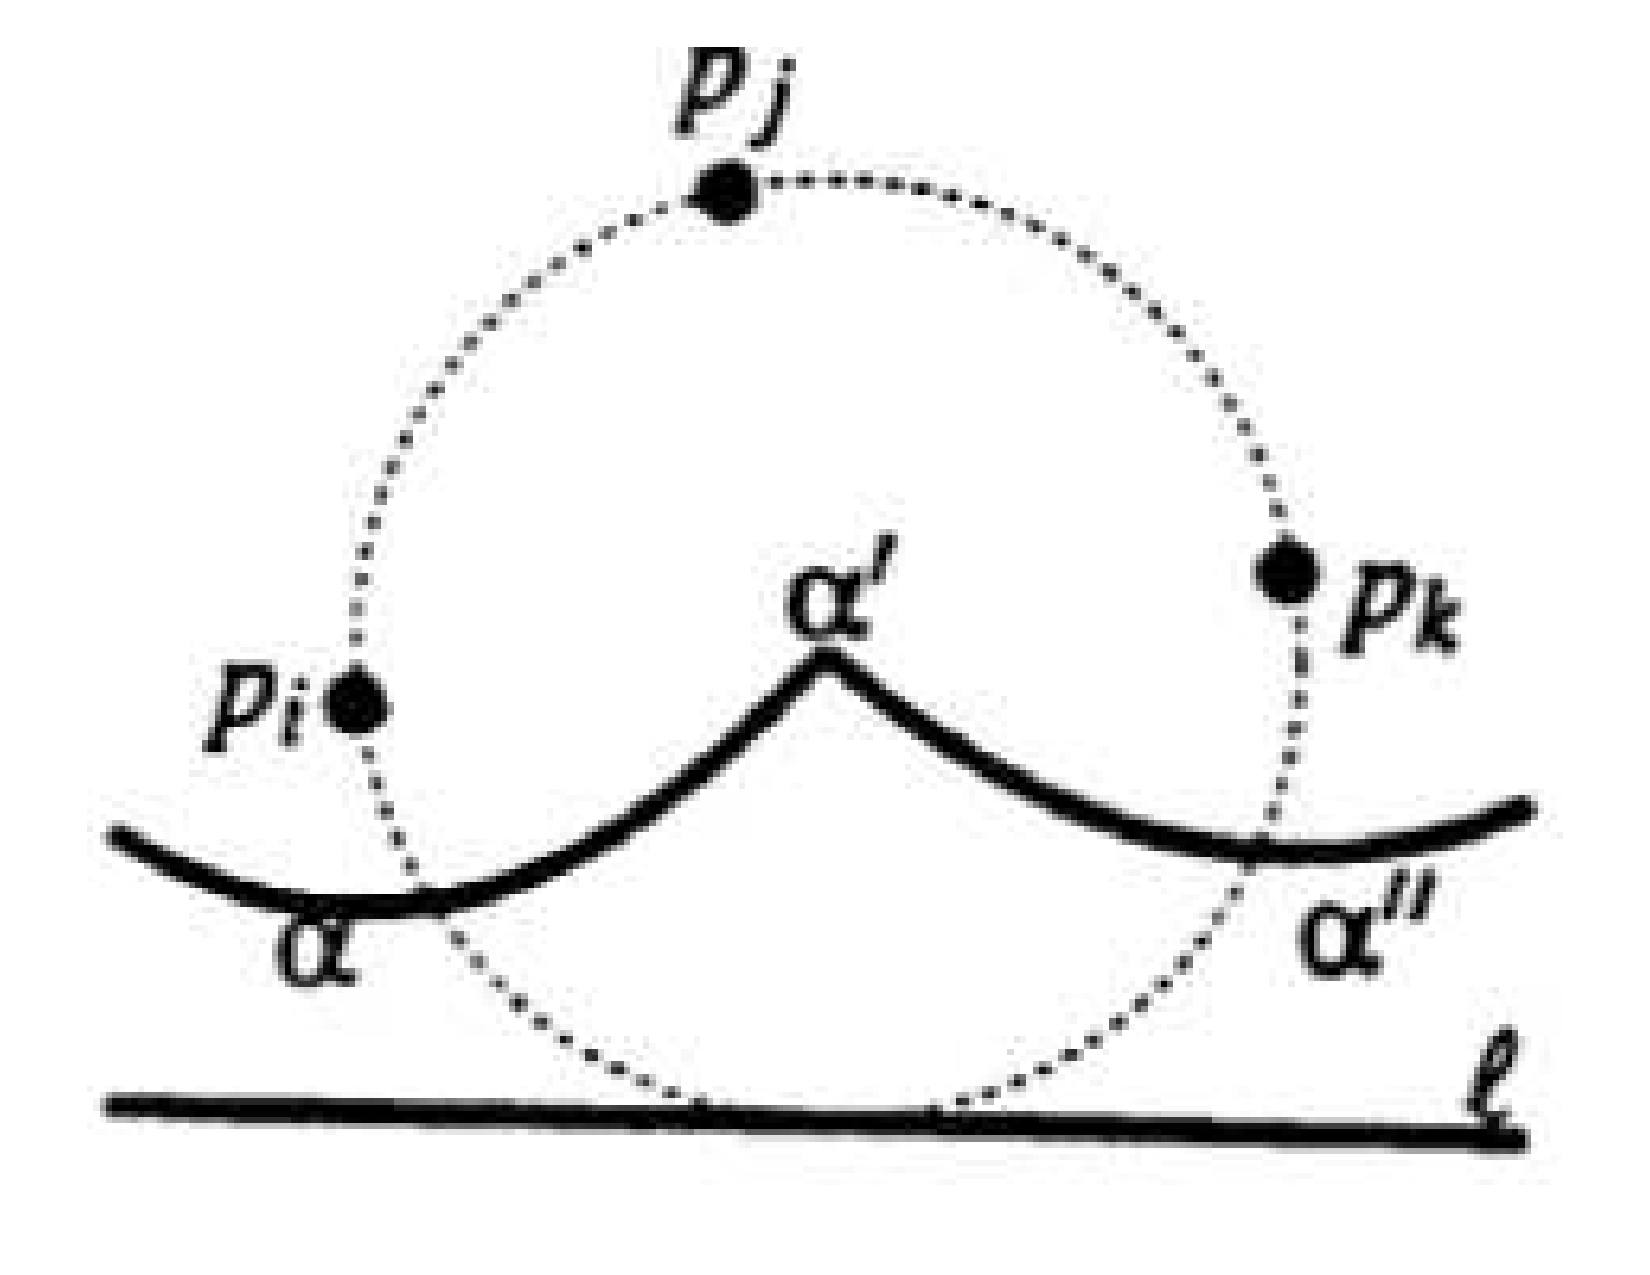
\includegraphics[width=50mm]{images/circle_event.pdf}
    \caption{Circle event. A circle with sites $pi$, $pj$ and $pk$ on its perimiter is tangent on the sweep line $l$, and a vertex $a'$  has been discovered in its centre.}
    \label{fig:circle_event}
\end{figure}

During the sweep, the algorithm maintains a so-called beach line. This is the curvy line just above the sweep line seen in Figure~\ref{fig:fortunes}. For each x coordinate the beach line consists of the lowest y value of any parabola. This means that the beach line consists of parabolic arcs, where each parabola can contribute to the beach line more than once.

It turns out that a circle event happens exactly when an arc of the beach line disappears because it is hidden by two neighbouring arcs. These two arcs will grow faster than a third arc, that ultimately degenerates to a single point, which forms the centre of the circle mentioned above.

\subsection{Point Location}
\subsubsection{Single Shot Algorithm}
The single shot algorithm takes as input a set of line segments forming a planar sub division. It answers queries of the same type as the point location algorithm to be explained in the next section but has a time complexity of O(n) meaning that it is not optimal. 

\paragraph{}
Basically, what the algorithm does is to locate the line segment lying directly below the query point in the cell. If the segments are stored in a DCEL, the segment that was found can then be used to trace out the rest of the cell. To find the segment, the algorithm runs through the whole list and iteratively tries to find a better candidate by looking at the coordinates of the end points. An optimal (and valid) candidate will lie below the query point and be closer to it than any other segment lying below it. 

\begin{figure}[]
    \centering
      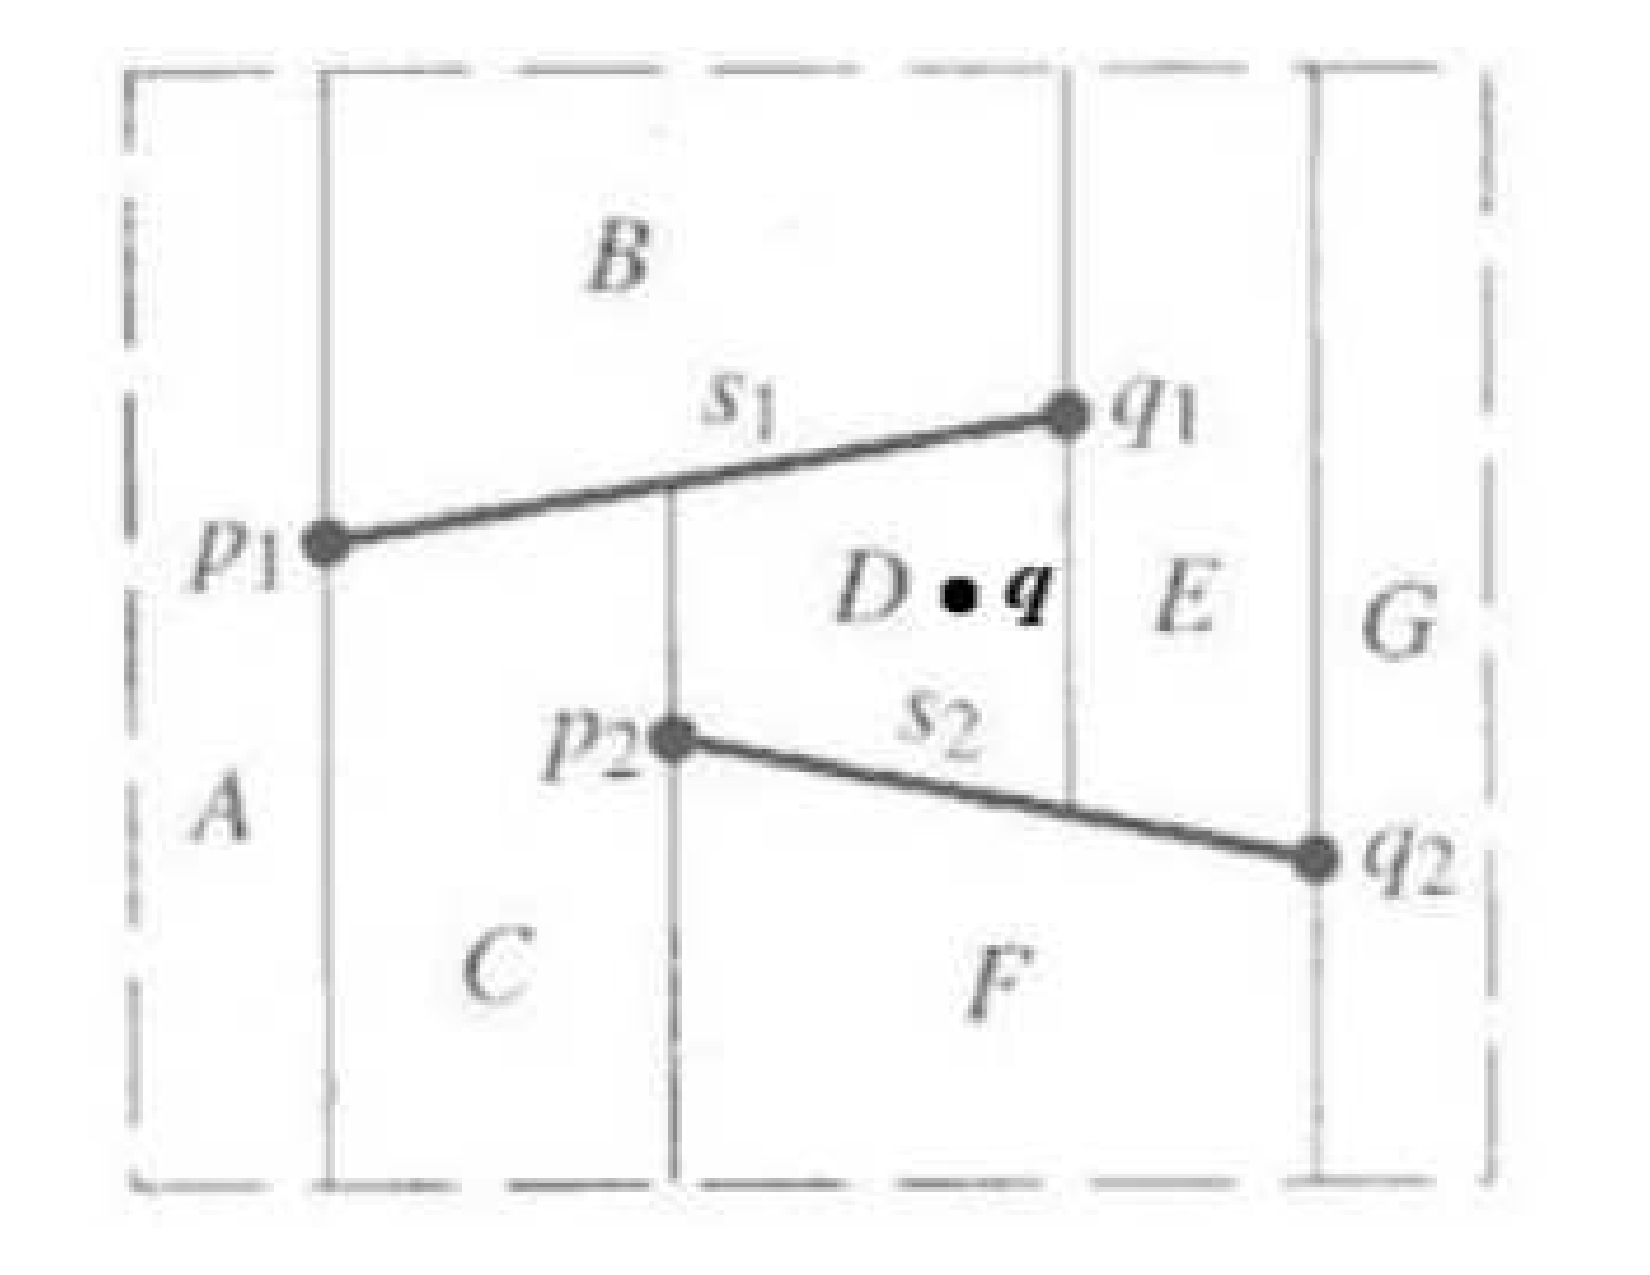
\includegraphics[width=50mm]{images/trapezoidal_map.pdf}
    \caption{A trapezoidal map inside a bounding box. Two line segments $s1$ and $s2$ have been inserted, which has generated a map of trapezoids $A$,$B$,$C$,$D$,$E$,$F$ and $G$. A query point $q$ is located in $D$.}
    \label{fig:trapezoidal_map}
\end{figure}

\subsubsection{Trapezoidal Map Algorithm}
The trapezoidal map algorithm takes as input a set of line segments forming a planar subdivision and outputs a trapezoidal map $T$ and a search tree $D$ that can be used to answer point location queries in O(logn) time. In return for the improved complexity, the algorithm will take O(nlogn) time to build the data structures. This is a desirable as we often want to perform several point location queries on the same map. 

\paragraph{}
Without modifications, the algorithm assumes that line segments are in general position. For a set of segments to be in general position they cannot cross each other (they can share an endpoint though) and no two distinct endpoints can lie on a vertical line.

\subsubsection{A trapezoidal map}
$T(S)$ of a planar subdivision represented as a list of segments S is created by erecting vertical lines (extensions) of each segment that stop when they hit an upper or lower segment. Each trapezoid of the resulting division will have one or two vertical sides and exactly two non-vertical sides. Since any vertical side of a trapezoid is created as an extension of an end point and no two endpoints can lie on a vertical line, a trapezoid can be uniquely represented as two points (left and right point) and two line segments (upper and lower boundaries). An example of a trapezoidal map can be seen in Figure~\ref{fig:trapezoidal_map}.

Two trapezoids are adjacent if the share a vertical side (an extension) and neighbours if they are adjacent and also share an upper or lower line segment. Any trapezoid in a trapezoidal map created from a set of line segments in general position can have at most 4 adjacent trapezoids and thereby at most 4 neighbours referred to as its upper left-, upper right-, lower left- and lower right neighbour. As an example, we can see in Figure~\ref{fig:trapezoidal_map} that the trapezoid $C$ has a $A$ as its lower left neighbour, $F$ as its lower right neighbour, and $D$ as its upper right neighbour.
\subsubsection{The search structure}
$D$ is a binary search tree that contains nodes representing the end point of a line segment (X nodes), the segment itself (Y nodes) or a trapezoid (leafs). Since the tree is assumed to be balanced (consult the references for an argument of why this is true), a trapezoid containing a query point can be found in O(logn) as a path from the root to a leaf. 

\begin{figure}[]
    \centering
      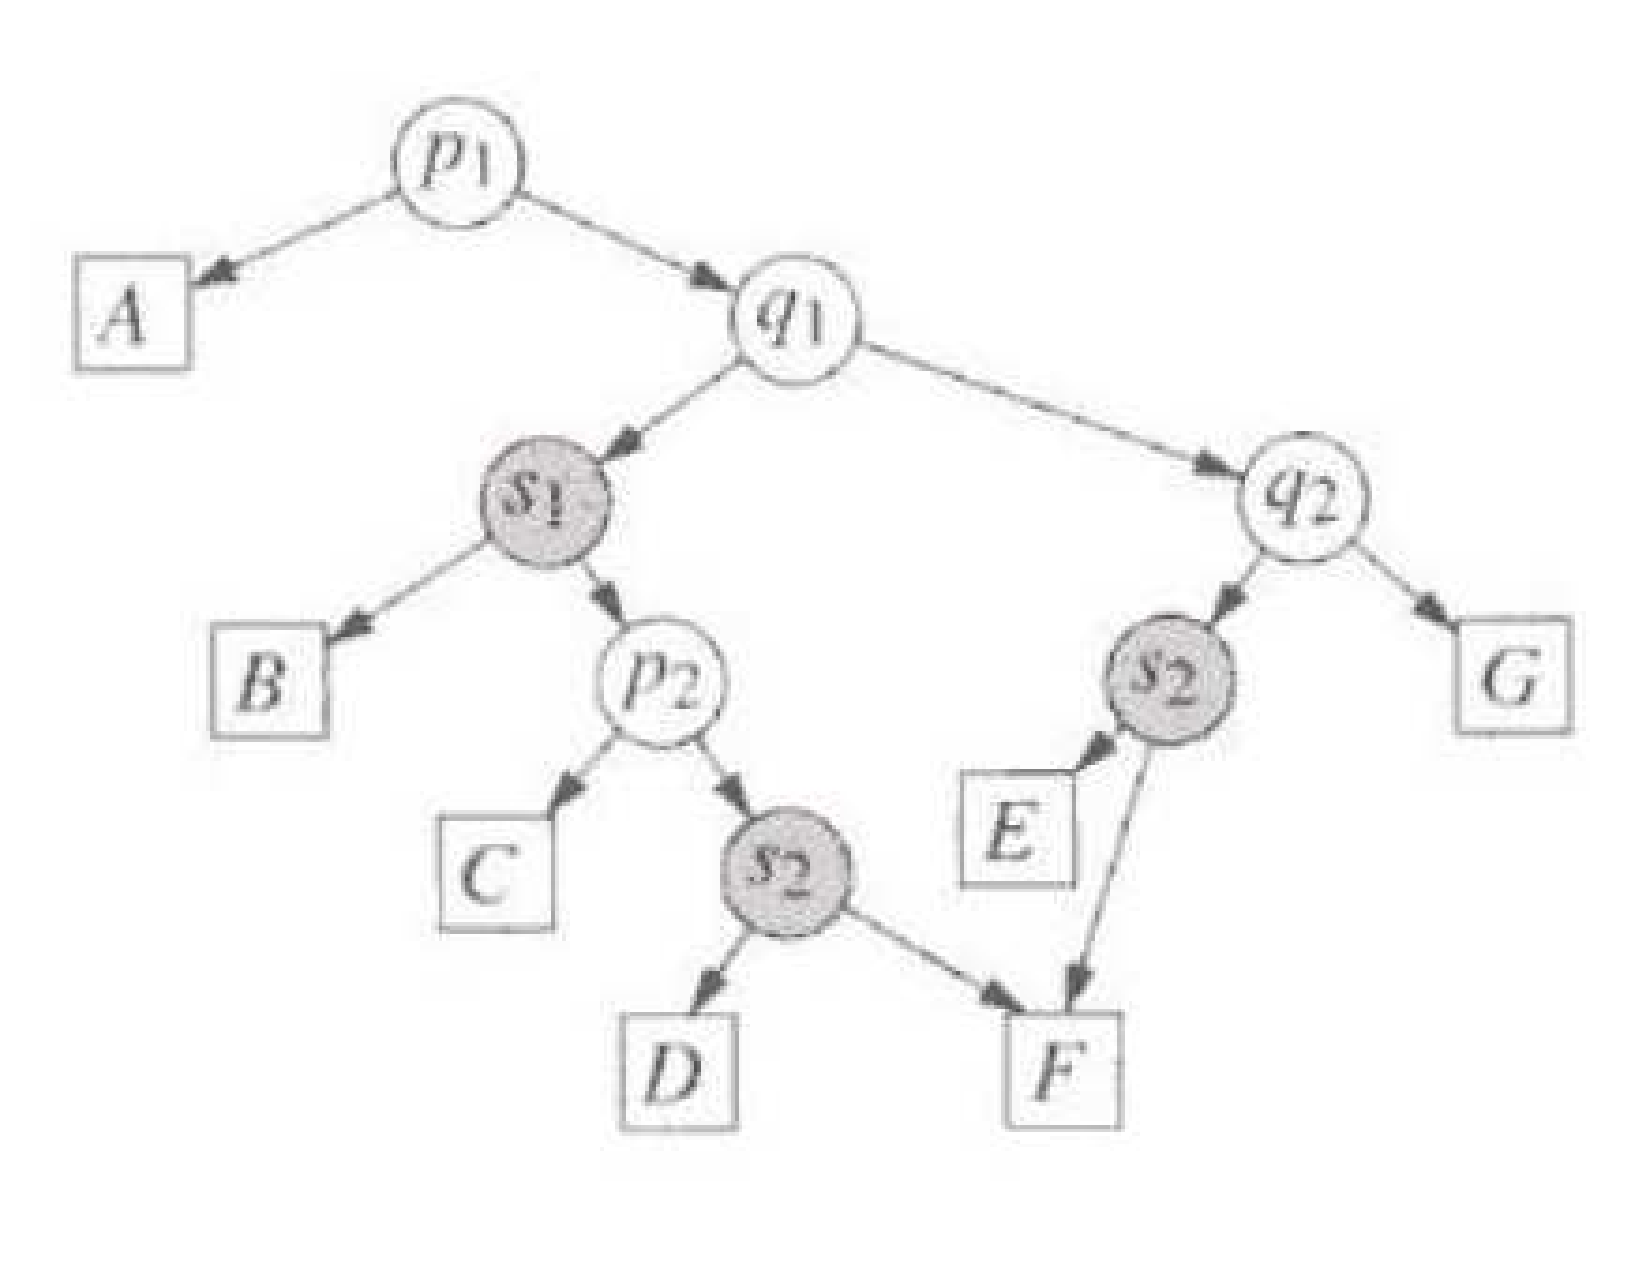
\includegraphics[width=80mm]{images/tree.pdf}
    \caption{A search tree with X nodes $p1$, $p2$, $p3$ and $p4$, Y nodes $s1$ and $s2$. The leaves are trapezoids $A$ to $G$. The search tree corresponds to the trapezodial map in Figure~\ref{fig:trapezoidal_map}.}
    \label{fig:tree}
\end{figure}

To find a path, one starts at the root and proceeds according to answers to questions varying with the type of node. At an X node, one proceeds in the left sub tree if the query point lies to the left of the end point that the node represents and right otherwise. At a Y node, one goes right if the query point lies below the line segment that the node represents and left otherwise.
The trapezoidal map algorithm is incremental in the sense that it starts with a blank map and a search tree containing only a single leaf (the rectangle or trapezoid that bounds the map). It then adds one edge to the map at a time and updates the search structures. To update the map, extensions are created from the end points of the newly added segment. If the segment intersects already existing extensions, these are shortened. To update the tree, the algorithm removes the leafs for the intersected trapezoids and adds leafs for the new ones that appear in the map.

In the case where a new segment is inserted and it spans multiple existing trapezoids, we have to create new trapezoids that may consist of merges of existing trapezoids. Using information about the neighbours, trapezoids can be merged in time linear in the number of trapezoids involved in the merge, which is assumed to be a constant operation. Furthermore,  the number of intersected trapezoids is not dependent on the number of segments in the input set. Updating therefore reduces to finding the left most intersected trapezoid. This can be done with a point location query in $D$ and the left most endpoint of the newly added line segment in O(logn) time. If the algorithm inserts $n$ segments, the global complexity of the algorithm will be O(nlogn)
%!TEX root = ./report.tex
\section{Problem Statement}
As mentioned in section, there are multiple useful applications of point location in voronoi diagrams. In the remainder of this report we describe a solution that facilitates this kind of point location using techniques from two algorithms that are known in advance – one that generates voronoi diagrams and one that performs point location in any planar subdivision. 

\subsection{Desirable Features}
\label{problem_analysis}

\begin{itemize}
  \item The complexity should be unchanged, i.e. not bigger than any of the existing algorithms
  \item The solution must be generic, i.e. not targeted a specific business area or domain
\end{itemize}

\subsection{Assumptions}
\label{assumptions}

\begin{itemize}
  \item We require that no two sites of the input share the same x-coordinate as this is a simplifying assumption made by the original point location algorithm. This assumption means that every trapezoid can be uniquely represented in terms of their left point, right point, bottom segment and top segment. Furthermore, every trapezoid can have at most four neighbours. It is clear that this assumption is unreasonable when working with real-world data. How to deal with input where such “degenerate” cases occur is described in \cite{computational_geometry}
\end{itemize}






%!TEX root = ./report.tex
\section{Solution}
The provided solution consumes a set of 2D points  $P$ and returns  $D$ for performing point location queries in a Voronoi diagram corresponding to $P$. The attached CD contains the implementation as C\# source code that builds against .NET 4.0. An example providing $P$ and querying $D$ can be found in the program main.  A parser and example for generating data points from  the geographical coordinates of a set of fast-food restaurants is included. 
\paragraph{}
The solution is based on the description provided in \cite{computational_geometry} on point location and Voronoi diagrams, and as such, we do not cover the everything in detail, but rather provide highligts of parts that we found to be tricky to get right.  The implementation of Fortunes algorithm is an open-source implementation that can be found at [cite to misc and codeplex project] . Also , the solution includes a simple GUI from [cise to misc and ref to other os project] that can be useed to visualize simple small-scale datasets.  The implementation of $T$ and $D$ is provided by the authors and our main work constitues in implementing these, besides bridging with Fortunes algorithm.
\paragraph{}
One way of accomplishing what we want would be to simply take to the output of Fortunes algorithm, that is, the generated edges, and give them as input to the algorithm for the trapezoidal map. Both algorithms run in O(nlogn)  so the the complexity of running the two in sequence is the same. Alternatively we could add the edges to $T$ on the fly as the are found by Fortunes. It is easy to see that we will get the same complexity as we are virtually doing the same thing. To show this easy connecting of the two algorithms, the implementation demonstrates the latter.

\subsection{Point location in Voronoi}
$D$ is implemented with a standard composite-pattern, and offers a $Find(point)$ operation that will return a bounding trapezoid for the query point.  Recall that a trapezoid is simply defined by its side points and top and bottom segment. And as each segment is just a segment w egot from the Voronoi diagram, it holds a reference to the site of the voronoi cell. Fortunes algorithm adds this edge to site reference, and, eventually, it is the only way that trapezoid can tell which Voronoi cells it lies in. Of course, queies will only be precise when all segments have been added, and all trapezoids are completely trapped inside Voronoi cells.
\paragraph{}
Each time a segment is discovered for the Voronoi diagram, it is inserted into the trapezoidal map, and $T$ is updated with new subtrees according to the new trapezoids that appear from the inserting the new segment. A this point a lot or re-wiring occurs, as new and existing trapezoids need to have their neighbourhoods re-wired correctly. One case of this is as seen in Figure~\ref{fig:contained_segment}. 

\begin{figure}[t]
    \centering
      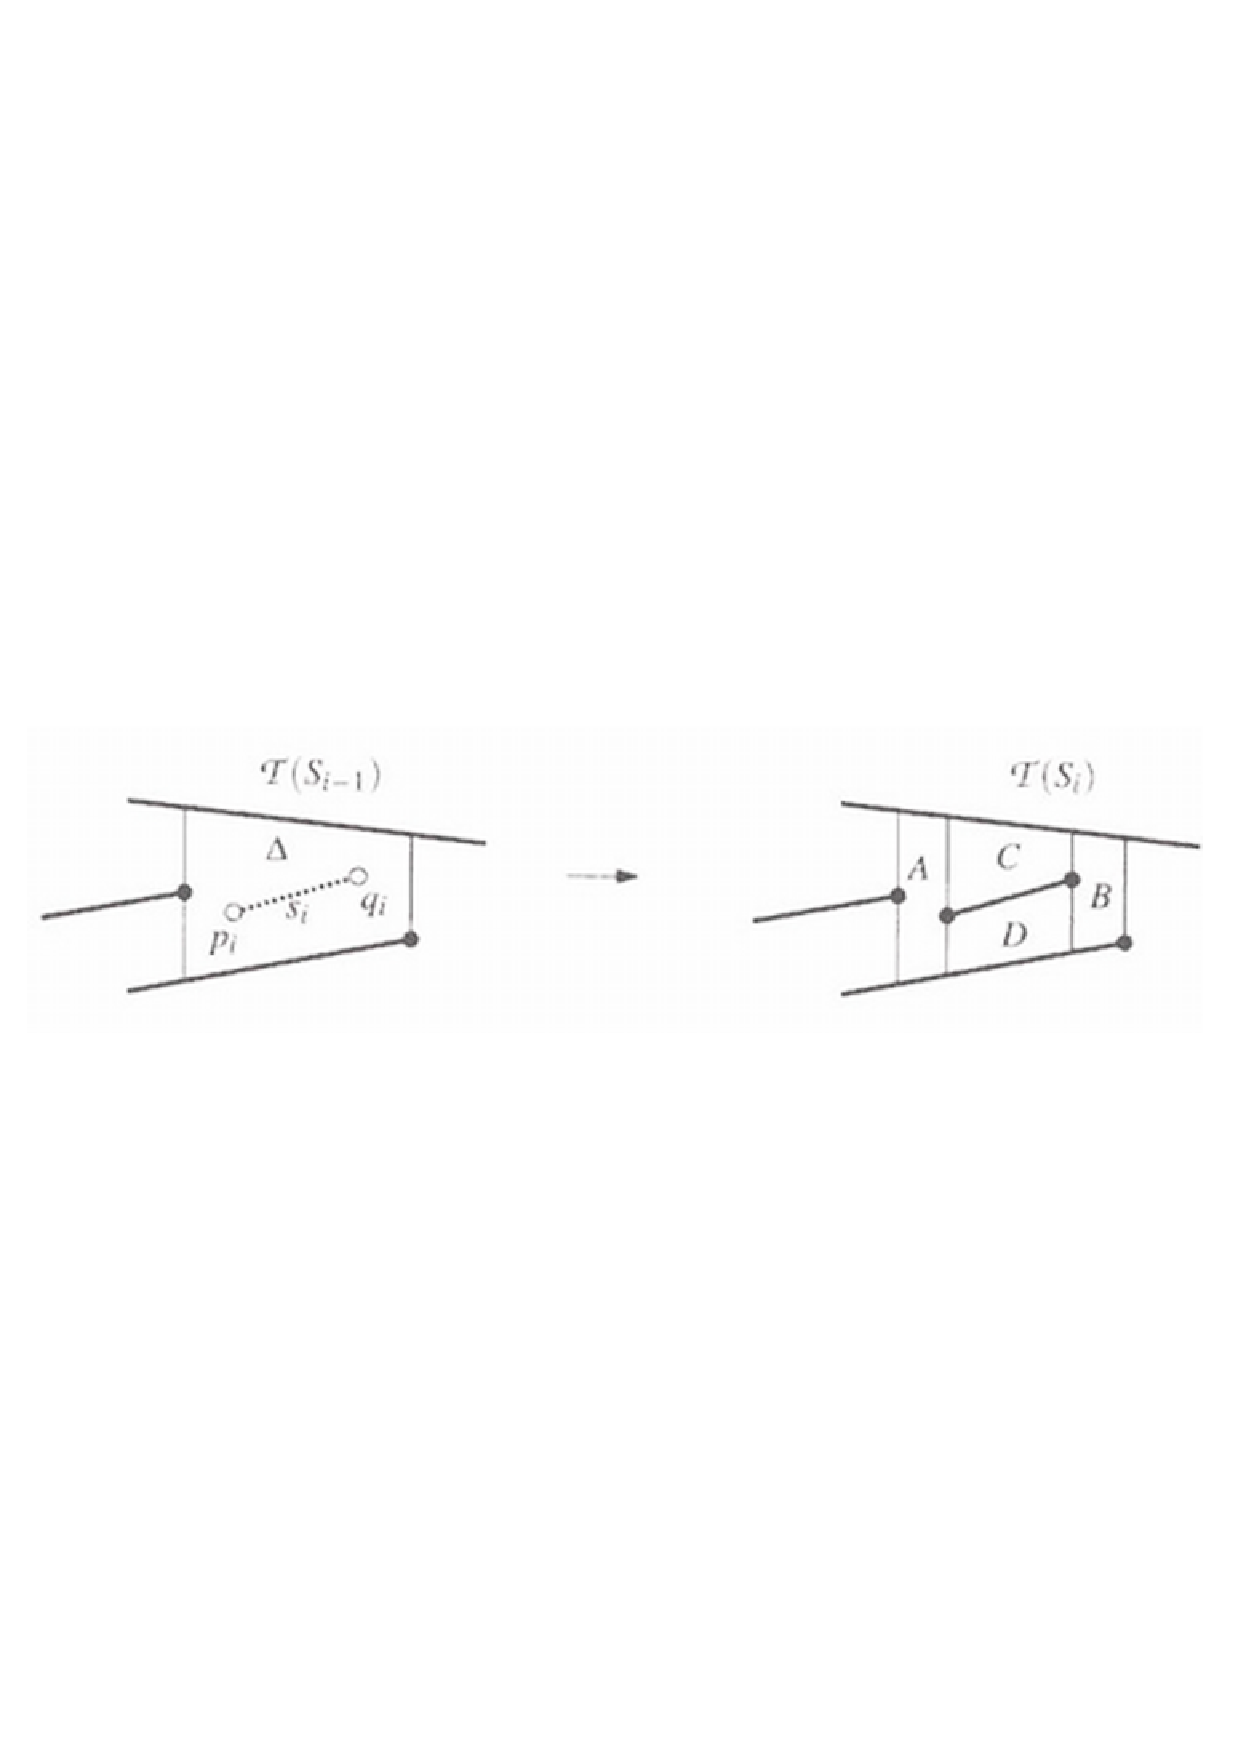
\includegraphics[height=80mm]{images/contained_segment.pdf}
    \caption{Inserting a segment in $T$ that is contained inside a single existing trapezoids}
    \label{fig:contained_segment}
\end{figure}

When the segment is contained in an existing trapezoid where we just need to make sure that we indetify what new trapezoids are created from inserting the segment, and updating $D$ with a corresponding subtree, which is somewat trival. In the case where a new segment crosses several existing trapezoids, things get a bit more tricky, and we will in the following explain how it can be solved.. The situation is depicted in Figure~\ref{fig:intersecting_segments}.\paragraph{}

\begin{figure}[t]
    \centering
      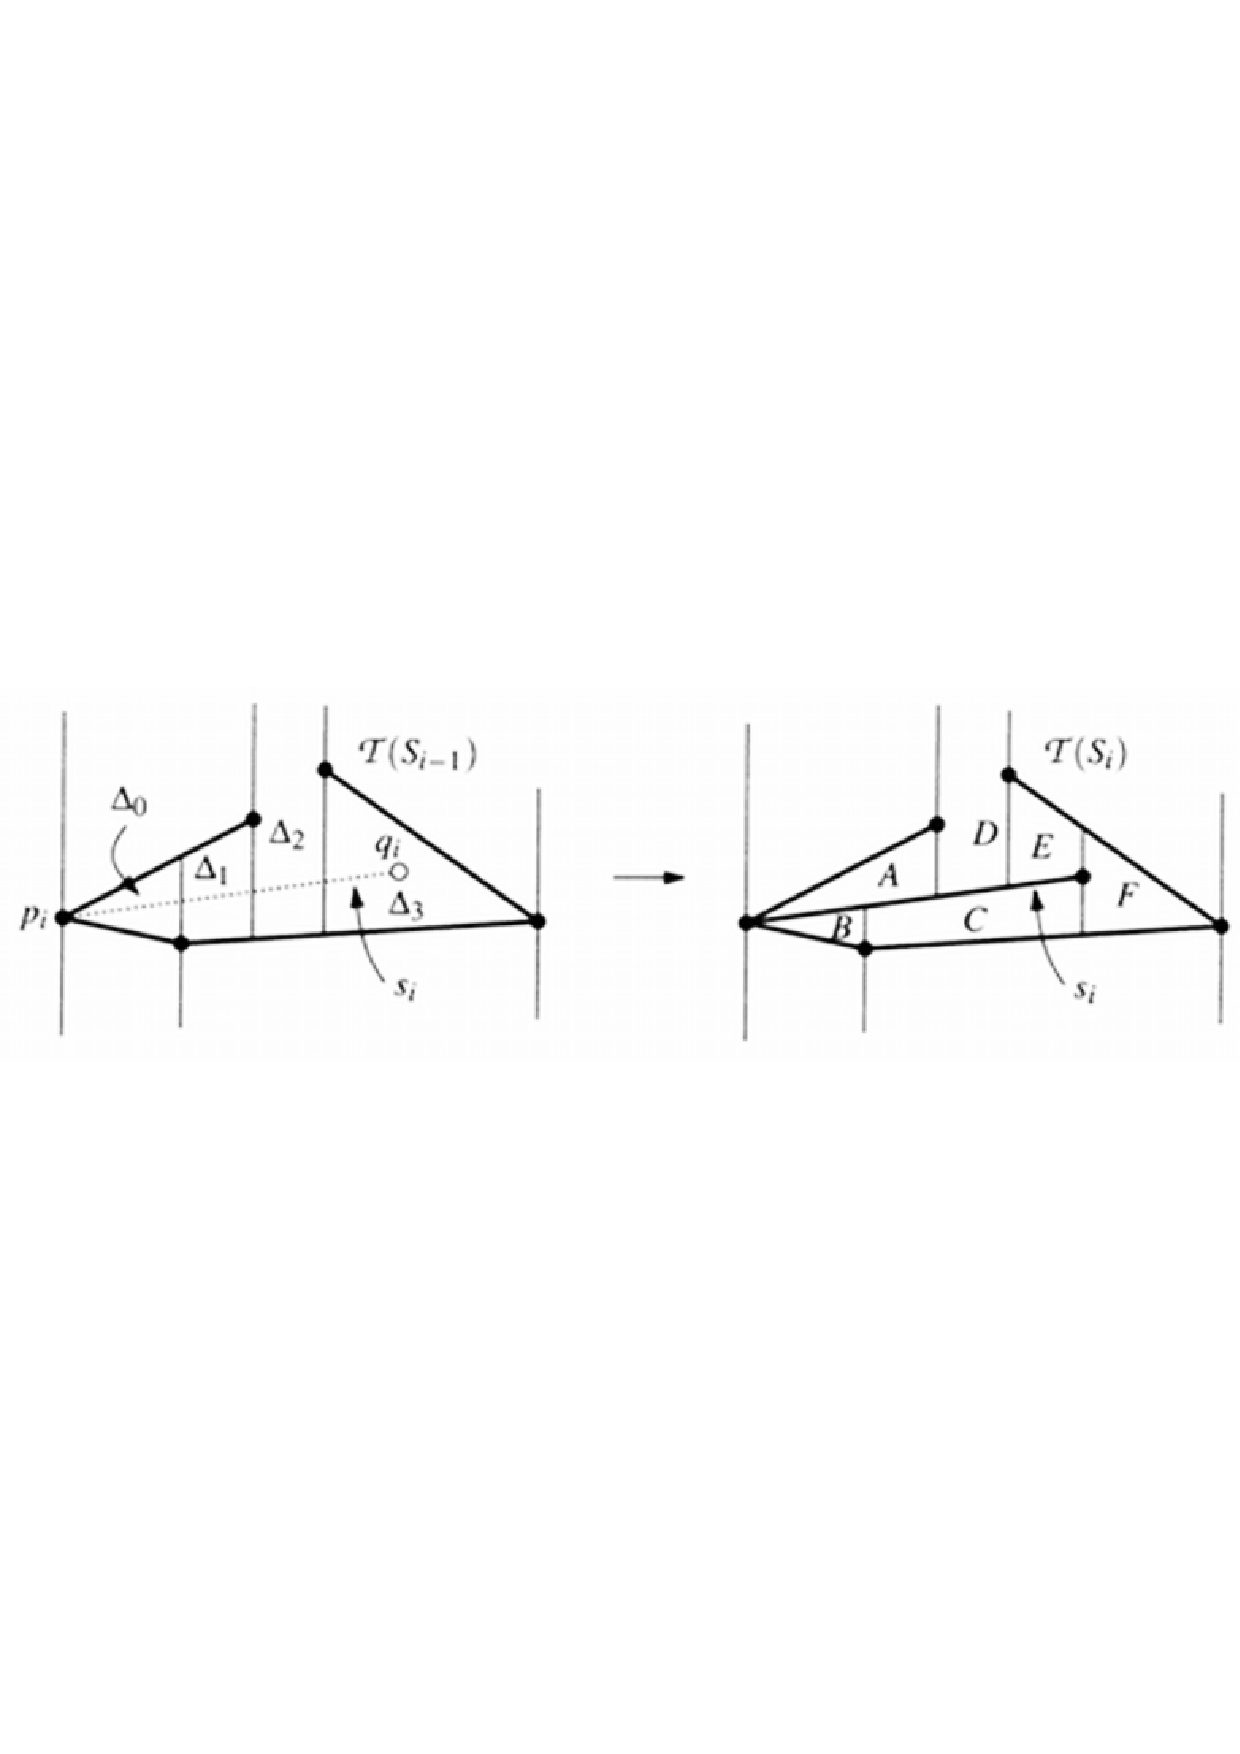
\includegraphics[height=80mm]{images/intersecting_segments.pdf}
    \caption{Inserting a segment in $T$ that crosses several trapezoids}
    \label{fig:intersecting_segments}
\end{figure}

\cite{computational_geometry} provides an good high-level description of how to handle this situation and states that it is done in linear time, which is possible as we can find neighbouring trapezoids by jumping from one trapezoid to the next by neighbour references - we do not need to look up neighbouring trapezoids in $D$. Now to handle the different case of the position of the inserted segment, we can start out by taking care of the boundries when one or both of the new segment's endpoints are connected to existing vertices, which is handled much like the the contained case. Secondly, we have to create new trapezoids that are, in some sense, horizontial merges of existing trapezoids. As an example, in Figure~\ref{fig:intersecting_segments}, we create  trapezoid $C$ with a left point from $\Delta 1$, a right point that will be the right most vertex of the newly inserted segment left most vertex, top being the new segment, and bottom being the the segment shared by  $\Delta 1$,  $\Delta 2$ and  $\Delta 3$.  Our solution to this is to always handle $\Delta 0$ and $\Delta 3$ in isolation, that is, add trapezoids much like with the case of the contained segment, and set the neighbourhoods. Secondly we do a recursive merge of the new trapezoids above the inserted segment, and under the segment. The pseudo code for doing an upper merge is show in Algorithm~\ref{alg:MERGEUPPER}.


\IncMargin{1em}
\begin{algorithm}
\label{alg:MERGEUPPER}
\SetKwData{Left}{left}\SetKwData{This}{this}\SetKwData{Up}{up}
\SetKwFunction{Union}{Union}\SetKwFunction{FindCompress}{FindCompress}
\SetKwInOut{Input}{input}\SetKwInOut{Output}{output}
\Input{A trapezoid $start$, a Segment $segment$, and a point $leftPoint$}
\Output{A list of trapezoids}
 \emph{Define LLN, ULN, LRN, URN as Lower Left Neighbour, Upper Left Neighbour, Lower Right Neighbour, Upper Right Neighbour of a trapezoid respectivly}\;
\Begin{
Create new trapezoid $t$\;
$t.leftPoint$ $\leftarrow$ $leftPoint$\;
$t.top$ $\leftarrow$ $start.top$\;
$t.bottom$ $\leftarrow$ segment\;
\BlankLine
$cur$ $\leftarrow$ $start$\;
\nl\While{$cur.rightPoint$ is below $segment$ and $cur$ is on the $segment$}{
	$cur$ $\leftarrow$ cur.URN;
}
\BlankLine
\nl\If{$segment.RightMostVertex.X$ $<$ $cur.RightPoint.X$}{
		$t.RightPoint$  $\leftarrow$ segment.RightMostVertex\;
	\lElse{
		$t.RightPoint$  $\leftarrow$ $cur.RightPoint$\;
	}
}
\BlankLine
\nl\If{$cur.rightPoint$ is before end of segment}{
        next $\leftarrow$ $MergeUpper(cur.LRN, segment,  cur.rightPoint)$\;
        $t.LRN$  $\leftarrow$ $next.First$\;
        $t.URN$ $\leftarrow$ $cur.URN$\;
}
 \Return{$t$ and $next$}\;
}
\caption{MergeUpper}\label{algo_disjdecomp}
\end{algorithm}\DecMargin{1em}

Doing a merge of the trapezoids below the inserted segment is done the same way, but with the neighbouring reference flipped horizontially. The last thing we need to do is to update $D$ with Algorithm~\ref{alg:INSERTMERGED}. One migt suspect that Algorithm~\ref{alg:MERGEUPPER} or Algorithm~\ref{alg:INSERTMERGED} could be in O(nlogn) in the number of segements and thus blow up the total running time, but as described in~\ref{background} this is not the case. Inserting a new segment is in O(logn). 

\IncMargin{1em}
\begin{algorithm}
\label{alg:INSERTMERGED}
\SetKwData{Left}{left}\SetKwData{This}{this}\SetKwData{Up}{up}
\SetKwFunction{Union}{Union}\SetKwFunction{FindCompress}{FindCompress}
\SetKwInOut{Input}{input}\SetKwInOut{Output}{output}
\Input{A list of existing trapezoids $olds$, a list of upper merged trapezoids $upper$, and a list of lower merged trapezoids $lower$, and the inserted $segment$}
\KwResult{Updated search tree $D$}
\Begin{
let $i$ $\leftarrow$ $j$ $\leftarrow$ $k$ $\leftarrow$ 0\;
\BlankLine
\nl\While{$k$ $\textless$ $olds.Count$}{
\BlankLine
	\nl\While{$upper[j].RightPoint.X$ $\textless$ $olds[k].RightPoint.X$}{
		$j$ $\leftarrow$ $j$ + 1\;
	}
\BlankLine
	\nl\While{$lower[i].RightPoint.X$ $\textless$ $olds[k].RightPoint.X$}{
		$i$ $\leftarrow$ $i$ + 1\;
	}
\BlankLine
	Replace $olds[k]$ with subtree of $segment$, $upper[j]$ and $lower[j]$ in $D$
\BlankLine
	$k$ $\leftarrow$ $k$ + 1\;
}
\BlankLine
}
\caption{InsertMergedTrapezoids}
\end{algorithm}\DecMargin{1em}

%Explain merge of cells situation, and maybe provide pseudo code of how we did it.
%Discuss implementaion dificulties, like updating neighbours, unprecise doubles in search tree.
%Porlbmees with voronoi implemenation, stuff that probably doesnt work with real fast food restaurant data set.

\subsection{Expected Customers}
%Expected number of hits by random shooting of points on the map. Chernoff expectation vs size of voron oi cells.


%!TEX root = ./report.tex
\section{Evaluation}
In order to test and evaluate the different parts of the project, we have created tests that check (1) the results of the merged algorithm and (2) our own isolated implementation of the trapezoidal map algorithm. We outline our test in this way to provide some confidence in the functionality of the overall solution and to identify the parts of it that are most likely to contain errors. 

Generally, we divided the tests into two categories and created an automated test case and a couple of static ones. Common to all test cases is that they feed a number of sites to the algorithm (or a number of line segments depending on the algorithm to be tested), performs a number of point location queries on the resulting search structure and compares the result to the expected output.

\subsection{Fortune’s algorithm}
We did not spend a lot of time testing the implementation of Fortune’s algorithm since we know its output is only valid to a certain degree. Using the GUI tool that came with the algorithm, we can see that line segments close the boundaries of the diagram are not included in the output. This means that the Voronoi diagram is corrupted and that a cell neighbour to the boundaries of the diagram can contain more than one site. This is a serious error that obviously causes a certain number of the failures in our tests.

\subsection{Automated test}
We created an automated test case that generates 1000 sites with random coordinates lying in the interval of [1-10.000] on both axis and feeds it to the merged algorithm. Since any site in a Voronoi diagram should obviously return its own Voronoi cell when used as query point in the search tree, this is exactly how we perform our test.

Due to fact that the merged algorithm check each line segment before it adds it to trapezoidal map, we know that the input set is in general position. On the other hand, if line segments that are not in general position occur, these will be removed from the Voronoi diagram and corrupt it even more. Still we can run our automated tests on any number of sites and get a success rate of approximately 20\% when perform the point location queries using the generated sites. This result is obviously not good but it is also not insignificant considering that the Voronoi diagram can potentially be seriously corrupted. 

Knowing that the implementation has trouble with generation of edges along the boundaries of the diagram it is also an interesting observation that the success rate of the automated tests tend to increase when we sort out query points from the problem areas.\paragraph{}

To convince ourselves that a substantial amount of the errors arise inside the implementation of Fortune’s algorithm, and in the filtering of the segments, we have tested our own implementation in an isolated environment 

\subsection{Static test}
While an automated test can generate a great amount of random test cases, we can only perform point queries with the sites from the input as these are the only points we can be sure to the know the Voronoi cells to. In the context of a trapezoidal map, we can generate random line segments and enforce their validity as input but we can’t write a procedure to check the output.

In order to evaluate the quality of our implementation of the trapezoidal algorithm, we have constructed a couple of limited and short test cases whose output have been manageable to check manually. Each test case contains a set of line segments forming a complete and valid Voronoi diagram and a number of query points who returned a correct result in each case. Besides these very small test cases, we invested a great deal of time in making sure that we handled the representation of the data structures, the representation of trapezoids (with pointers to neighbours etc.) and the search tree correctly.
Furthermore, we have run our implementation of the trapezoidal map algorithm many times during the last phases of development with successful results, so we are fairly confident that it works as intended.

The original thought was to run a final test experiment on a real world data set of fast food restaurants in the US. This proved not to be possible as the implementation of Fortune’s algorithm overflowed the stack after approximately 10.000 records of input. While it would be valuable to assert the applicability of the algorithm on a real world data set, we believe that the results from the remaining tests are good enough on their own. We find that the trapezoidal map algorithm seems promising enough combined with a better implementation of Fortune’s algorithm. 



%!TEX root = ./report.tex

\section{Threats to Validity}

While we believe that our evaluation ultimately makes a valuable and sufficient test of the solution for the scope of this project, there are a couple of possible threats to validity.

\subsection{Internal Threats}

\begin{itemize}
	\item In the current set up we apply our solution to 5 data sets of limited size whose results are manageable to deal with outside the algorithm. They all produced a correct result which provides a great deal of confidence in the correctness of the implementation. A better test would, however, involve more test cases.

	\item Our solution is constructed from two separate and real-world algorithms for point location and Voronoi diagram generation. We implemented point location in C\# and found an implementation of Fortunes Algorithm online written in .NET 1.0. During the project we discovered that the latter implementation, in its original form, contained errors and that some Voronoi cells of the output contained two or three sites instead of just one.

\paragraph{}
These erroneous cells are very small in number and always occur in positions adjacent to the boundaries of the diagram. The consequence of the error to our final product is that a lookup in the search tree with a query point contained in an erroneous cell will return a random site. In a real-world scenario the impact from this threat would be major but for the scope of this project we believe it is minor as we have identified the error and take it into account when designing our test cases.
\end{itemize}

\subsection{External Threats}

\begin{itemize}
	\item An ambiguity appears when performing point locations with query points that lie exactly on a line segment or a vertex. Reading through the literature listed in the references to this report, certain solutions are mentioned. Still we choose not to take this case into account since the assumption that line segments are in general position seems reasonable for the scope of this project and we still handle a pair of other similar ambiguities.

\paragraph{}
The general position assumption is however much less reasonable in the context of fast food restaurants as data from the real world is non-controllable. Therefore, not handling this case infers some restrictions on the generalizability of our results in a real world context which is a threat to validity. 

\end{itemize}
        
           
%!TEX root = ./report.tex
\section{Plan For Future Work}
\subsection{Future Work}
\label{sec:future_work}
Create a clean and generic voronoi implementation in .NET 4.x
Find best point for planar location. Not trivial, would probably be Hawaii, but that would
be winning a lot of oceanic area.
\subsection{Something else?}


%!TEX root = ./report.tex
\section{Conclusion}
We have outlined the main ideas behind Fortunes algorithm for generating Voronoi diagrams, and an algorithm for generating trapezoidal maps. The solution provided demonstrates how this can be done and we have discussed a few central challanges in implementing the algorithm. Once we understand the underpinnings of the two algorithms, making them work in combination is almost trivial and we have a point location time in O(logn). The we have presented is implemented in a generic fashion and it should be easy to see the solution used on top of other data sets.
\paragraph{Acknowledgements}
We would like to thank Rasmus Pagh for encouringing us to explore a new area, and introduce us to two exiting algorithms. We also want to thank him for a course full of learningful lectures, and on-the-spot guidance and support for this project.  
%!TEX root = ./report.tex
\bibliography{report}

%% Old bibliography
% %
% % ---- Bibliography ----
% %
% \begin{thebibliography}{99}
% %

% \bibitem[3]{2mich:tar}
% Michalek, R., Tarantello, G.:
% Subharmonic solutions with prescribed minimal
% period for nonautonomous Hamiltonian systems.
% J. Diff. Eq. 72, 28--55 (1988)

% \bibitem[4]{2tar}
% Tarantello, G.:
% Subharmonic solutions for Hamiltonian
% systems via a $\bbbz_{p}$ pseudoindex theory.
% Annali di Matematica Pura (to appear)

% \bibitem[5]{2rab}
% Rabinowitz, P.:
% On subharmonic solutions of a Hamiltonian system.
% Comm. Pure Appl. Math. 33, 609--633 (1980)


% \end{thebibliography}


\end{document}









